\begin{figure*}
\begin{center}

\begin{minipage}{\linewidth}
\begin{subfigure}[b]{\linewidth}
\begin{minipage}{0.5\textwidth}
\begin{center}
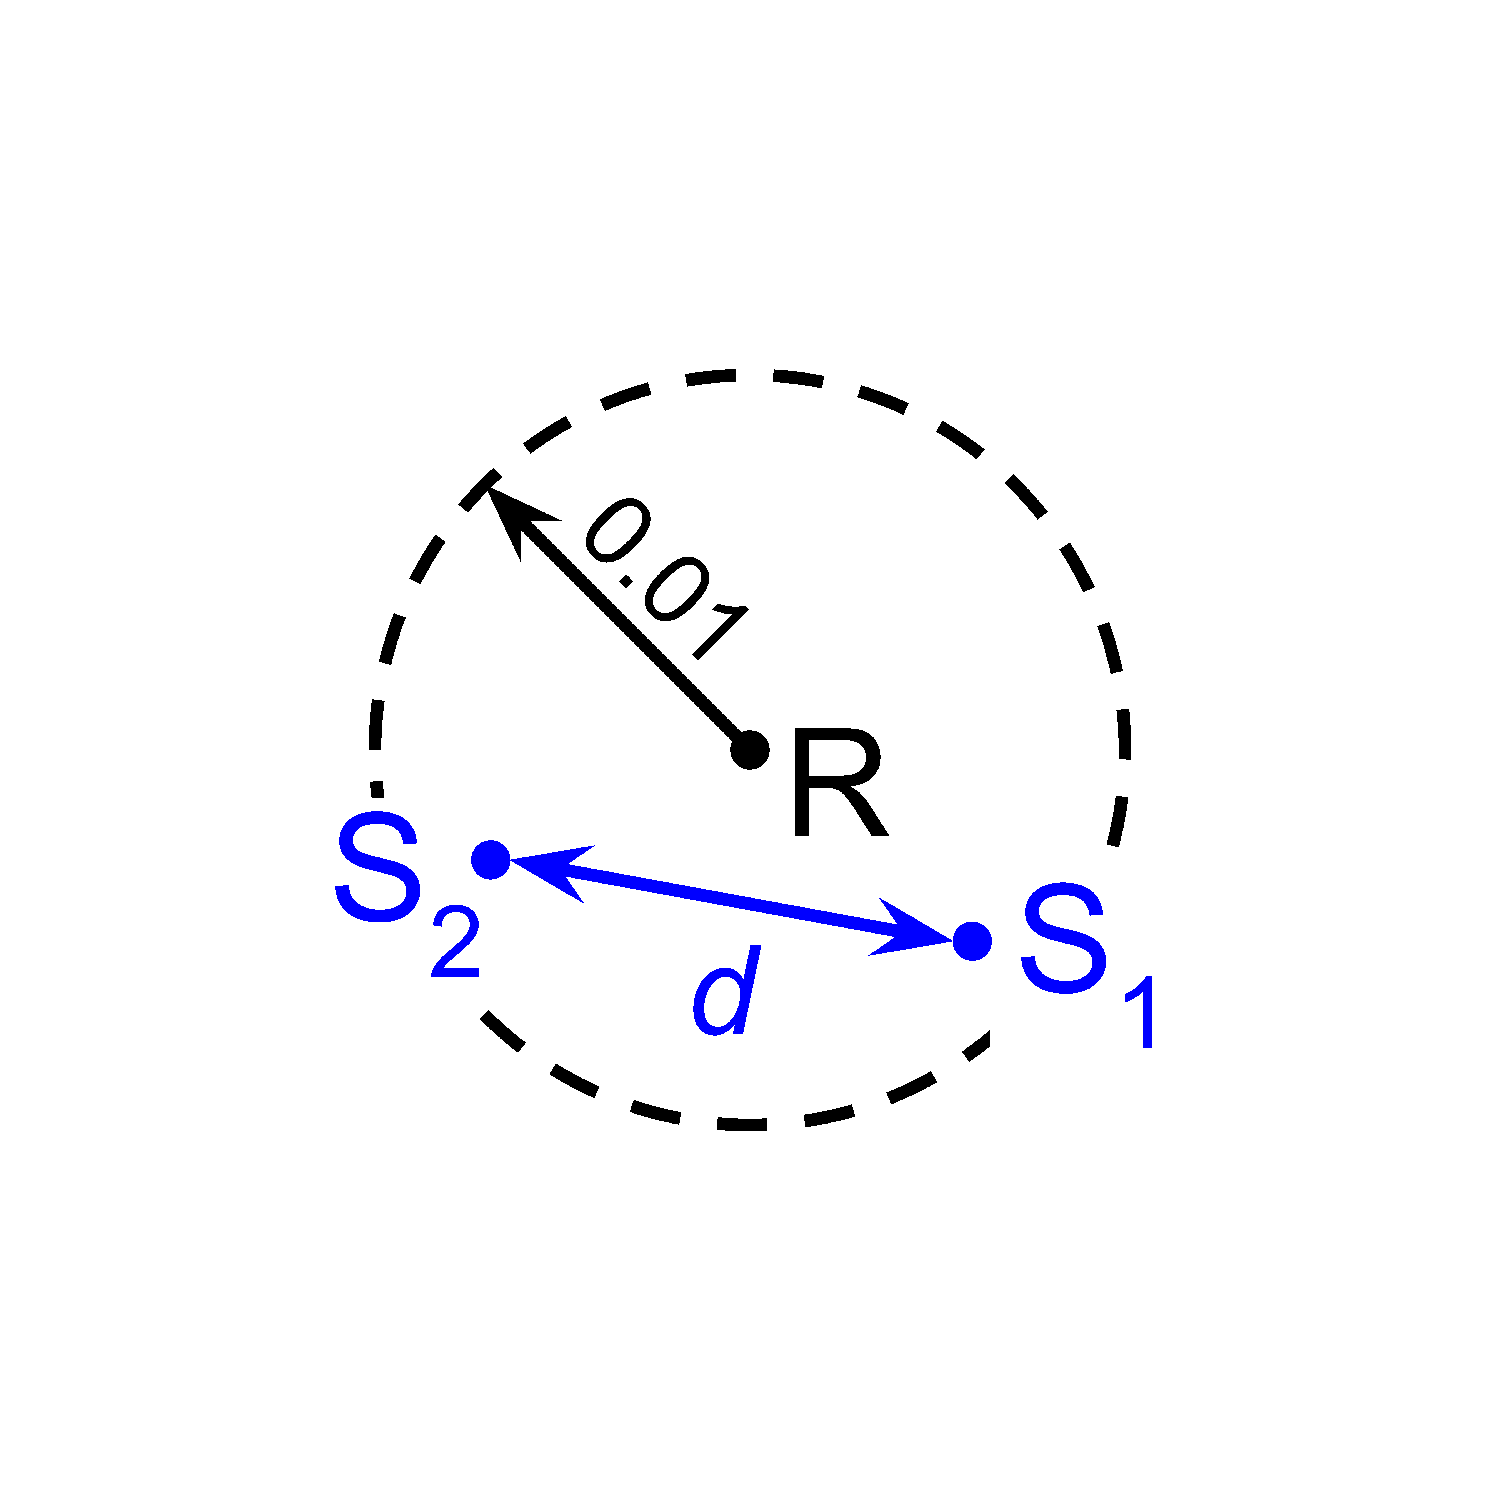
\includegraphics[width=0.5\linewidth,trim=5cm 5cm 5cm 5cm, clip]{dimensionality-statistic}
\end{center}
\end{minipage}%
\begin{minipage}{0.5\textwidth}
\caption{
Sampling process used to evaluate similarity constraint.
}
\label{fig:dimensionality_measure}
\end{minipage}
\end{subfigure}
\end{minipage}
\begin{subfigure}[b]{\linewidth}
\begin{minipage}{0.6\linewidth}
\includegraphics[width=\linewidth]{sphere/bitweight=0dot5+seed=1+title=dimensionality_barplot+_data_hathash_hash=c0f6c5cf854ff253+_script_fullcat_hash=03ce1e318a24a109+ext=}
\end{minipage}
\begin{minipage}{0.35\linewidth}
\caption{
Mean similarity constraint.
Error bars represent 95\% confidence intervals.
}
\label{fig:sphere_barplot}
\end{minipage}
\end{subfigure}
\begin{minipage}{\linewidth}
\begin{subfigure}[b]{\linewidth}
\centering
\includegraphics[width=\linewidth]{sphere/bitweight=0dot5+seed=1+title=dimensionality_distnplot+_data_hathash_hash=c0f6c5cf854ff253+_script_fullcat_hash=03ce1e318a24a109+ext=}
\begin{minipage}{0.8\textwidth}
\caption{
Distribution of sampled similarity constraint values, where each horizontal sliver represents one independent observation.
}
\label{fig:sphere_distnplot}
\end{minipage}
\end{subfigure}
\end{minipage}

\caption{
Similarity constraint of tag-matching metrics.
}
\label{fig:sphere}

\end{center}
\end{figure*}
